\chapter{Systemanalyse}\label{chapter:systemanalyse}
Systemanalysen har til formål at finde frem til hvilke procedurer og data der skal bruges til at udforme en løsning af problemet.
Først præsenteres systemdefinitionen, som har udgangspunkt i problemformuleringen og de funktionaliteter der blev opstillet i \myref{section:interview2}.
Efterfølgende vil der være henholdsvis en analyse af problemområdet og anvendelsesområdet, som sidst i kapitlet vil danne baggrund for en kravspecifikation.

\section{Systemdefinition}
På baggrund af \myref{chapter:problemanalyse} udarbejdes en BATOFF-analyse, som beskrevet i OOA\&D\citep{OOA&D2001}, og efterfølgende formuleres en systemdefinition baseret på disse kriterier.

Denne analyse har til formål at definere retningen for det videre arbejde i projektet.
Systemdefinitionen er en kort tekst, der har til formål at beskrive systemets overordnede krav og funktionaliteter.

Nedenfor ses BATOFF udarbejdelsen og efterfølgende systemdefinitionen.
BATOFF kriterierne hjælper med at danne et overblik over diverse emner, som en systemdefinition bør omfatte.

\subsection{BATOFF}
\begin{description}
\item [Betingelser]\hfill
\begin{itemize}[nolistsep,noitemsep]
\item Adgang til tilbud
\item Interesse for indkøb, opskrifter og tilbud
\end{itemize}

\item [Anvendelsesområde]\hfill
\begin{itemize}[nolistsep,noitemsep]
\item Tilbud
\item Brugere
\item Servere
\item Klienter
\item Overvågning af tilbud
\item Midler til lagring af data
\item Styring af anbefalinger
\end{itemize}

\item [Teknologi]\hfill
\begin{itemize}[nolistsep,noitemsep]
\item Smartphone (Mobil web-device)
\item Tablets
\item Til udvikling: Computer m/udviklerværktøjer
\item Browser m/internetadgang
\end{itemize}

\item [Objekter]\hfill
\begin{itemize}[nolistsep,noitemsep]
\item Opskrifter
\item Indkøbsvarer (tilbud)
\item Brugere
\item Vurdering
\item Præferencer
\item Indkøbsliste
\item Tilbudsaviser
\end{itemize}

\item [Funktioner]\hfill
\begin{itemize}[nolistsep,noitemsep]
\item Overvågning af tilbud
\item Håndtering af indkøbslister
\item Bedømmelse af opskrifter
\end{itemize}

\item [Filosofi]\hfill
\begin{itemize}[nolistsep,noitemsep]
\item Indkøbsassistent og inspirationsgenerering
\end{itemize}
\end{description}



\subsection{Konkret systemdefinition}\label{Sysdef}

Systemet hjælper på problemer, der kan opstå i forbindelse med indkøb og madlavning i hjemmet.
Systemet organiserer indkøbslister, opskrifter og aktuelle tilbudsvarer, samt anbefaler opskrifterne, baseret på bedømmelser af opskrifter og præferencer angående madvarer.
Aktuelle tilbud hentes fra internettet, og kan tilføjes, sammen med generiske varer, til indkøbslister.
Desuden kan det overvåge hvornår, en valgt generisk vare kommer på tilbud.
Systemet tilgås via en webbrowser, således det kan bruges på både computer, tablet og smartphone.
Systemet udvikles som en serverside-applikation med adgang til databaser til håndtering af system- og brugerdata.
Udviklingen af systemet kræver computere med de relevante udviklingsværktøjer.

Denne systemdefinition vil nu være udgangspunkt for vores videre arbejde i rapporten.

\section{Modellering af System}
Ifølge OOA\&D analyseres både problemområdet og anvendelsesområdet for problemet\cite[s. 6]{OOA&D2001}.
Disse er defineret som følgende:

\textit{\textbf{Problemområde:} ''Den del af omgivelserne, der administreres, overvåges eller styres ved hjælp af et system''}

\textit{\textbf{Anvendelsesområde:} ''En organisation, der administrerer, overvåger eller styrer et problemområde''}

\subsection{Problemområdet}
Problemområdet bruges som en modellering af et problem fra den virkelige verden, hvor et system skal benyttes for at administrere, overvåge eller styre et område. 
Dette gøres ved at beskrive diverse klasser, som vil indgå i systemet, ud fra disse ses på hvilke hændelser, som er involveret i klasserne.
Ydermere ses der på, hvilken adfærd der er mellem diverse klasser, hændelser og objekter i systemet.
Dette giver en beskrivelse af, hvilken opførsel og struktur problemområdet skal modellere.
I dette projekt omfatter problemområdet planlægning af indkøb, inspiration til mad samt det at spare penge ved at købe tilbud.
For at beskrive dette nærmere, ses der på klassediagrammer og hændelsestabeller, for at danne overblik over systemet og ende ud med en sammenhængende model for problemområdet.
\subsection{Anvendelsesområdet}
Hvor problemområdet beskriver systemet, beskriver anvendelsesområdet, hvordan systemet skal anvendes.
Ud fra dette spørgsmål opstilles en række af krav for systemets funktioner og grænseflade.
Til dette formål ses der på brugen af systemet, hvilke typer af brugere der er, hvilke brugsmønstre der er for de individuelle funktionaliteter i systemet, samt hvordan funktionaliteterne skal tilgås fra grænsefladen.
I dette projekt indebærer anvendelsesområdet at kunne administrere sine indkøb, få en let oversigt over tilbud, finde inspiration til mad i form af opskrifter, samt at kunne overvåge varer, som man har interesse for at købe på tilbud.


\section{Analyse af problemområde}

Ud fra systemdefinitionen i \myref{Sysdef} ved vi, at systemet skal holde styr på følgende:

\begin{itemize}[noitemsep,nolistsep]
	\item Tilbud
	\item Varer
	\item Indkøbslister
	\item Opskrifter
\end{itemize}

Med disse informationer kan systemet hjælpe brugeren til at finde billige varer i bestemte butikker og eventuelt anbefale opskrifter, der bruger disse tilbudsvarer.
I de følgende afsnit vil disse emner blive beskrevet vha. klassebeskrivelser, en hændelsestabel, og et klassediagram.

\subsection{Klasser}
I dette afsnit vil vi analysere klassernes sammenhæng, derudover vil yderligere klasser blive tilføjet, hvis det findes nødvendigt.

\begin{description}
\item[Vare]\hfill\\
En vare indgår i opskrifter, og indkøbslister.
Når man laver sin indkøbsliste, kan man vælge varer man vil købe, og tilføje dem til indkøbslisten.
Desuden kan en vare have et antal tilbud, hvilket betyder, at der også skal laves en relation til tilbudsklassen.

\item[Tilbud]\hfill\\
Når der kommer nye varer på tilbud, modelleres disse og kobles, vha. en association, til varer.

\item[Opskrift]\hfill\\
En opskrift har en liste over ingredienser, hvilket altså er varer samt mængden af varen.
I interviewene i \myref{section:interview2}, blev det nævnt, at brugerne gerne ville kunne vurdere en opskrift og dermed få anbefalet yderligere opskrifter, som minder om denne.
For at kunne lave vurderinger, skal der laves en vurderingsklasse.

\item[Vurdering]\hfill\\
En vurdering med tal gives for at rangere opskrifter. 
Vurderingen danner også grundlag for, at systemet kan anbefale opskrifter.

\item[Anbefaling]\hfill\\
En anbefaling, af en opskrift, kan gives til personer, når de har givet positive vurderinger af andre opskrifter, som minder om den vurderede opskrift.

\item[Person]\hfill\\
Personklassen gør det muligt at holde styr på forskellige personer, da disse tilsluttes opskrifter, vurderinger, og indkøbsliter.
Derudover vil en person også have præferencer, for butikker de handler i, samt madvarer.

\item[Indkøbsliste]\hfill\\
Indkøbslister laves af en person, og fyldes op med objekter fra vareklassen.
Indkøbslisterne kan deles imellem flere brugere.
\end{description}


\subsection{Hændelser}\label{handelser}
På baggrund af de nævnte funktionaliteter i prototype interviewene, \myref{section:interview2}, er der fundet forskellige hændelser, relevante for funktionaliteterne.
Ud fra disse laves en hændelsestabel, der beskriver, hvilke klasser forskellige hændelser påvirker.
Formålet med, at identificere hændelserne samt at analysere disse i en hændelsestabel, er at forstå problemområdet bedre.
Derved kan det hjælpe med forståelsen for, hvordan en løsning ville kunne designes, for at afhjælpe de problemer, der findes i problemområdet. 
Desuden kan tabellen hjælpe med strukturen på klasserne.
Hvis to klasser har samme hændelser, kan disse klasser ofte tilpasses under én klasse, og dermed opnås en bedre struktur.

\begin{table}[H]
  \centering
    \colorlet{shadecolor}{gray!40}
    \rowcolors{1}{white}{shadecolor}
      \begin{tabular}{l|lccccccc}
      %\hline
       								& \rot{Tilbud}  & \rot{Indkøbsliste} & \rot{Opskrift} & \rot{Vare} & \rot{Person}& \rot{Vurderinger} \\ \hline
      Vare tilføjet til indkøbsliste&               & +      &          & +     & +     &   \\ 
      Vare fjernet fra indkøbsliste	&              	& +      &          & +     & +     &   \\ 
      Vare aftjekket på indkøbsliste&               & +      &          & +     & +     &   \\ 
      Opskrift valgt ???       		& +             & +      &          & +     & +     &   \\ 
      Tilbud oprettet        		& +            	& +      & +        & +     &       &   \\ 
      Tilbud aktiveret        		& +            	& +      & +        & +     &       &   \\ 
      Tilbud udgået          		& +        		& +      & +     	&       &       &   \\ 
      Vare tilføjet til overvågning & +          	&        &          & +     & +     &   \\ 
      Vare fjernet fra overvågning  & +          	&        &          & +     & +     &   \\ 
      Overvågningsvare på tilbud    & +  			&		 &			& + 	& +		&	\\
      Del indkøbsliste       		&               & +      &          &       & +     &   \\ 
      Indkøbsliste oprettet  		&              	& +      &          &       & +     &   \\ 
      Indkøbsliste slettet  		&             	& +      &          &       & +     &   \\ 
      Vurdering givet				&             	&        & +        &       & +		& + \\
      Anbefaling givet				&				&		 & +		&		& +		& + \\
      
    \end{tabular}
  \caption{Hændelsestabel. Viser hvilket klasser, problemområdets hændelser påvirker.}\label{tabel:haendelsestabel}
\end{table}


Hændelsestabellen, i \myref{tabel:haendelsestabel}, viser både, hvilke hændelser der findes i problemområdet, samt hvilke klasser de påvirker.
Et \textbf{+} beskriver en hændelse, som forekommer højest en gang i et hændelsesforløb.
En \textbf{*} beskriver hændelser, der kan forekomme flere gange i et hændelsesforløb.\citep{OOA&D2001}
På tabellen kan det ses, at klasser der bliver påvirket af mange hændelser, er klasser som \textbf{Indkøbsliste}, \textbf{Vare} og \textbf{Person}.

Ud fra hændelsestabellen kan der dannes et overblik over klassernes interne interaktion, samt hvilke hændelser der involverer hvilke klasser.
Denne information kan vi nu bruge til at lave en struktur over klasserne i problemområdet.

\newpage
\subsection{Struktur}\label{sec:struktur}
\begin{figure}[h]
	\centering
		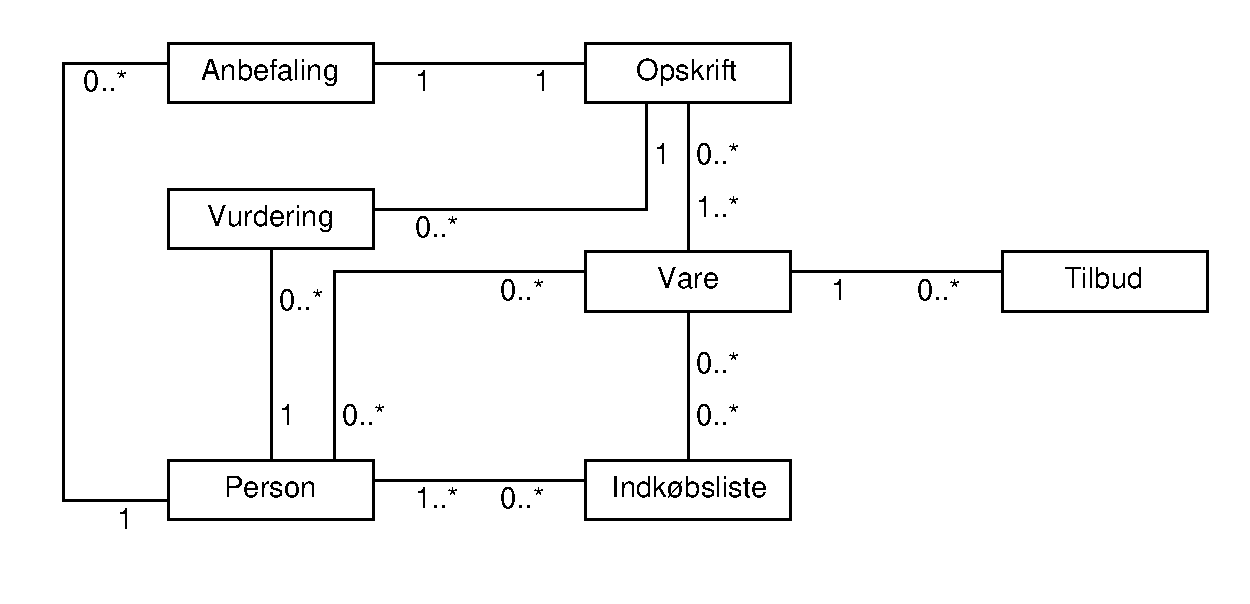
\includegraphics[scale=0.6]{images/Diagrams/klassediagram_model_simple.pdf}
	\caption{Klassediagram over problemområdet.}\label{figur:PDklasse}
\end{figure}

Klassediagrammet som ses på \myref{figur:PDklasse}, beskriver forholdet mellem de forskellige klasser som findes i problemområdet.
Diagrammets sammenhænge er dannet ud fra hændelsestabellen, og beskrivelserne af klasserne.\fxnote{Sørg for at denne model stemmer over ens med modellen vi ender ud med i programmet. I programmet kan vi så henvise til at denne model over klasserne blev brugt til at danne associationerne, imellem klasserne. Der er nemlig ingen henvendelse lige pt, og det kan helt klart bruges. Beskrivelsen nedenfor er næsten identisk med den man finder i Arkitektur - Søren}

Personer kan lave indkøbslister, disse indkøbslister kan være ejet og administreret af enten en eller flere personer.
En indkøbsliste kan bestå af nul til mange varer.
En vare kan være på tilbud i mere end en butik, og derfor have nul til mange tilbud.
En vare kan desuden indgå i en opskrift, og er derfor forbundet med nul til mange.
Desuden har opskrifterne en til mange varer på listen over ingredienser.
Varen kan også være tilføjet til overvågningslisten hos en person, så derfor har personer og varer en nul til mange relation på hinanden.
En person i problemområdet kan give hver opskrift en vurdering, derfor kan personen give nul til mange vurderinger.
En vurdering gives til en opskrift alene, imens en opskrift kan have mange vurderinger, eller ingen vurderinger.
Anbefalinger består af en opskrift, imens personen kan modtage nul til mange anbefalinger.

Ovenstående analyse vil hjælpe til at designe systemets implementering, først foretages dog en analyse af anvendelsesområdet, for at undersøge hvad der er muligt at foretage sig i systemet.

\section{Analyse af anvendelsesområdet}\label{sec:anvendelses}
Dette afsnit tager udgangspunkt i metoder fra ''Objektorienteret Analyse og Design'' og benytter disse til at analyserer anvendelsområdet, dette omfatter brug af systemet, funktioner i systemet samt grænsefladen der er tilknyttet.\citep{OOA&D2001} 
Afsnittet skal give et overblik over funktionaliteten af systemet, samt formidle hvordan brugeren interagere med systemet.

\subsection{Brug}
Denne del af analysen har til formål at fastlægge interaktion mellem systemet og aktører.
Dette gøres ved at identificere brugsmønstre for aktørerernes aktioner i systemet.
\subsubsection*{Aktører}
I dette IT-system er der blevet identificeret to aktører. 
Den første værende datakilden, eTilbudsavisens API, hvor tilbudende hentes fra og den anden værende de brugere, som benytter systemet.
For disse to aktører er der således udarbejdet en aktørtabel \myref{aktortabel}, der giver overblik over hvilke brugsmønstre der er, samt hvilke aktører der er relevante for disse.

\begin{table}[h]
\centering
    \colorlet{shadecolor}{gray!40}
    \rowcolors{1}{white}{shadecolor}
\begin{tabular}{rcc}
%\hline
				    & Bruger               		& eTilbudsavis  \\ \hline
Login               & \cmark                    & 		 		\\
Listehåndtering     & \cmark                    & 		 		\\
Søgning             & \cmark                    & 				\\
Indstil præferencer & \cmark                    & 				\\
Vurder opskrift     & \cmark                    &  	   			\\
Se anbefalinger     & \cmark                    & 				\\
Hent tilbud         &  						    & \cmark 		\\ \hline
\end{tabular}
\caption{Aktørtabel. Viser hvilke aktører er involveret i hvilke brugsmønstre}\label{aktortabel}
\end{table}

\subsubsection*{Bruger}

\textbf{Formål:} En person, som ønsker at bruge en eller flere af IT-systemets funktionaliteter, til at hjælpe med planlægning af mad og indkøb.

\textbf{Karakteristik:} Systemets brugere har meget varierende erfaring med IT-systemer, samt er bredt ud over mange forskellige aldersgrupper, majoriteten er dog mellem 18 - 30 år og har middel erfaring med IT.

\textbf{Eksempler:}Bruger A er en 21-årig universitetsstuderende, som for nyligt er flyttet hjemmefra. A har meget erfaring med IT, og bruger det dagligt til at navigere rundt på internettet. 
A har let ved at navigerer rundt i systemet og bruge dets funktionaliteter til at lave besparelser på det allerede lave budget, samt at undgå at få pasta med ketchup til aftensmad hver dag.

Bruger B er en 47-årig familiefar, der kun har smartphone, da det er arbejdstelefonen på givet af arbejdet. 
B benytter systemet til at handle ind på vej hjem fra arbejde, hvor indkøbslisten lavet af konen eller datteren bruges som guide i supermarkedet. 
B vil således gerne kunne tilgå listen fra telefonen, så der ikke er behov for at kører hjem og hente den på papirsformat.

\subsubsection*{eTilbudsavisen}

\textbf{Formål:} eTilbudsavisen har til formål at gøre tilbudsdata tilgængelig for systemet, dette sker igennem API.
Dette giver information om navnet på tilbudet, pris, periode, butik og meget andet.
Da dataene der hentes igennem API'et kan være af meget svingende kvalitet, filtreres det, så kun forståeligt tilbudsdata kommer igennem.

\textbf{Karakteristik:} eTilbudsavisen er pålidelig med dataene der sendes, kvaliteten af dataene kan dog svinge meget, og eTilbudsavisen tilbyder ingen fleksibilitet i dets arbejde, hvilket resulterer i noget ubrugeligt data som filtreres fra.

\textbf{Eksempel:} eTilbudsavisen gør 2.000 tilbud tilgængelig, heri er nogle på et format der ikke klargøre hvad der er på tilbud, men blot giver en række mærkenavne som er på tilbud.
En sådan uforståelig række bliver filtreret ud såvel som andre uforståelige tilbud, og systemet ender tilbage med 1.337 brugbare tilbud, der kan vises til brugeren.

\subsubsection*{Brugsmønstre}
For en yderligere beskrivelse af de funktionaliteter i systemet, som vedrører en given aktør, modelleres en række brugsmønstre, dette er de samme brugsmønstre som ses i aktørtabellen i \myref{aktortabel}. 
Hver enkelt af disse mønstre vil blive beskrevet igennem en brugsmønstrespecifikation. 
Det er ikke alle mønstre som ses på denne liste, nogle af disse er sammentrækninger af flere andre mønstre, som alene virker simple og repetitive at beskrive. 
Andre er udeladt da de ikke passer helt ind i en sammentrækning, men variationen fra det mønster og andre brugsmønstre ellers beskrevet, er så minimal, at mønstret er anset som værende ubetydeligt at beskrive.

\subsubsection*{Brugeridentifikation}
\textit{Brugsmønster:} Brugeridentifikation sker ved at en bruger logger ind i systemet.
Brugeren vil blive præsenteret for en side hvor, e-mail og password kan indtastes.
Herefter godkender eller afviser systemet den indtastede data og håndterer resultatet, enten ved at logge brugeren ind, eller ved at give en fejlbesked.
Alternativt kan brugeren oprette en ny konto i systemet, ved oplysning af navn e-mail og password.
Hvis du ikke er logget ind i systemet kan du ikke tilgå systemets funktionaliteter.

\textit{Objekter:} Person.

\textit{Funktioner:} Registrer bruger, Log ind, Log ud.

\subsubsection*{Listehåndtering}
\textbf{Brugsmønster:} Dette brugsmønster dækker over indkøbslisten såvel som overvågningslisten.
Brugeren kan inden for listens brugsmønstre tilgå funktionaliteterne i vilkårlig rækkefølge, givet der er oprettet en liste på forhånd.
En bruger kan oprette, dele og slette sine egne indkøbslister.
Hvis en liste er delt med andre og prøver at slette denne, forlader brugeren listen frem for at slette den.
Overvågningslisten på den anden hånd, eksisterer altid og kan hverken oprettes eller slettes.
Brugeren kan på begge lister tilføje eller fjerne en vare.
Varerne på overvågningslisten er varer som brugeren er interesserede i at få tilbud om.
Når en vare på denne liste kommer på tilbud modtager brugeren en notifikation derom.
Ved indkøbslisten er der tre funktionaliteter til at tilføje ting til listen.
Man kan tilføje ingredienser fra en opskrift.
Ydermere kan en bruger aftjekke eller fjerne varer fra listen.

\textbf{Objekter:} Indkøbsliste, Overvågningsliste, Varer, Tilbud, Personer, Opskrifter.

\textbf{Funktioner:} Opret liste, Fjern Indkøbsliste, Tilføj til liste, Fjern fra liste, Aftjek på indkøbsliste, Del liste, Forlad Indkøbsliste.

\subsubsection*{Søgning}
\textbf{Brugsmønster:} Brugeren kan søge efter varer, hvorefter systemet filtrerer efter søgestrengen for at finde relevante resultater.
Dette brugsmønster benyttes flere steder, både til at søge på tilbud til sine varer, såvel som opskrifter.


\textbf{Objekter:} Vare, Tilbud, Opskrifter.

\textbf{Funktioner:} Søg efter tilbud, Søg efter opskrifter.

\subsubsection*{Tilpas præferencer}
\textbf{Brugsmønster:} 
Brugere i systemet har mulighed for at fravælge madvarer eller butikker, som vises i programmet.

\textbf{Objekter:} Varer.

\textbf{Funktioner:} Sæt Præferencer, Filtrer efter præferencer.

\subsubsection*{Opskrifts håndtering}
\textbf{Brugsmønster:}
Brugeren kan interagere med opskrifter på forskellig vis. 
Som bruger har man mulighed for at oprette, klone, ændre, slette og vurdere opskrifter.
Når en opskrift oprettes vil brugeren bedes tilføje instruktioner, tid og ingredienser.
En bruger vil have mulighed for at ændre i sine egne opskrifter, og ligeledes kunne kopiere andres opskrifter og derefter tilføje ændringer i disse.
Fra ingredienslisten på en opskrift kan brugerne tilføje en eller flere varer til deres indkøbslister, samt skalere ingredienslisten til et bestemt antal personer, så brugerne får købt den rigtige mængde.
Brugerne har også mulighed for at vurdere opskrifter, ud fra brugerens vurderinger, vil systemet anbefale nye opskrifter til brugeren.

\textbf{Objekter:} Opskrift, Vurdering, liste af vurderinger, varer, indkøbsliste.

\textbf{Funktioner:} Se opskrift, oprette opskrift, ændre opskrift, klone opskrift, vurder opskrift, tilføj vare til liste, skalering af opskrift, slette opskrift.

%\subsubsection*{Vurder}
%\textbf{Brugsmønster:}
%Efter en opskrift er vurderet, kan andre brugere se den gennemsnitlige vurdering af en opskrift, og de brugere som har vurderet opskrifter, vil få anbefalet opskrifter som ligner.
%
%\textbf{Objekter:} Opskrift, Vurderinger, Liste af vurderinger.
%
%\textbf{Funktioner:} Vurder opskrift.

\subsubsection*{Se anbefalinger}
\textbf{Brugsmønster:} Brugeren kan se foreslåede opskrifter ud fra tidligere vurderede opskrifter.

\textbf{Objekter:} Opskrift, Vare.

\textbf{Funktioner:} Send anbefaling.

\subsubsection*{Hent tilbud}
\textbf{Brugsmønster:} Dette brugsmønster igangsættes af systemet, der periodisk henter tilbud fra eTilbudsavis og gemmer dem i systemet.

\textbf{Objekter:} Tilbud.

\textbf{Funktioner:} Hent tilbud.


\subsubsection{Funktioner}

I dette afsnit beskrives funktionerne der skal bruges for at kunne håndtere hændelserne fra problemområdet, og brugsmønstrene beskrevet ovenfor. 
Der findes fire typer funktioner: Aflæsnings-, opdaterings-, beregnings-, og signaleringsfunktioner.\citep{OOA&D2001}
Først identificeres funktionerne, hvorefter der gives en kategori til funktionerne, og en bedømmelse af deres kompleksitet. Herefter gives en kortfattet beskrivelse af funktionen hvor dette er tilstrækkeligt, ellers gives en dybere beskrivelse.

\begin{table}[H]
  \centering
    \colorlet{shadecolor}{gray!40}
    \rowcolors{1}{white}{shadecolor}
      \begin{tabular}{l|lllll}
      %\hline
      \textbf{Funktioner}			& {Kompleksitet}	& {Kategori}  	\\ \hline
      Log ind						& Medium			& Beregning, Opdatering		\\
      Log ud						& Simpel			& Opdatering	\\
      Registrer bruger				& Simpel			& Opdatering	\\
      Tilføje varer til lister		& Simpel       		& Opdatering	\\ 
      Fjerne varer fra lister		& Simpel       		& Opdatering	\\ 
      Oprette og slette lister		& Simpel       		& Opdatering	\\ 
      Dele lister					& Medium       		& Opdatering	\\ 
      Søgning på tilbud for varer   & Medium     		& Beregning		\\ 
      Sætte præferencer				& Simpel       		& Opdatering	\\ 
      Filtrere for præferencer		& Kompleks     		& Beregning		\\ 
      Give vurdering				& Simpel       		& Opdatering	\\ 
      Sende anbefaling				& Meget kompleks	& Aflæsning, signalering, beregning		\\ 
      Meddele tilbud på varer		& Medium      		& Signalering	\\ 
	  Se opskrifter					& Simpel       		& Aflæsning		\\ 
	  Se tilbud						& Simpel       		& Aflæsning		\\ 
      Hente tilbud					& Simpel	       	& Opdatering	\\           
    \end{tabular}
  \caption{Funktionstabel. Viser de forskellige funktioner der skal bruges, samt deres kompleksitet og kategori.}\label{tabel:functionstable}
\end{table}

\textbf{Log ind:} Her bliver sendt brugerinformationer, som verificeres med brugerne registreret i systemet. 
Hvis dette fuldføres, opdateres modellen således brugeren er registreret som værende logget ind.

\textbf{Log ud:} Brugeren der før var logget ind, opdateres til at være logget ud.

\textbf{Registrer bruger:} En ny bruger sender sine brugerinformationer, og et nyt login oprettes i modellaget.

\textbf{Tilføje varer til lister:} Denne funktion skal tilføje et objekt af vare klassen til en indkøbsliste, eller en overvågningsliste.

\textbf{Fjerne varer fra lister:} Funktionen her skal så fjerne disse objekter igen.

\textbf{Oprette og slette lister:} Denne funktion bruges når en indkøbsliste skal oprettes således man kan tilføje varer til denne.

\textbf{Dele lister:} Skal opdatere modellen således en anden bruger kan tilgå samme indkøbsliste som brugeren der deler sin liste. 

\textbf{Søgning på tilbud for varer:} Søger efter tilbud som passer til varen der søges for.

\textbf{Sætte præferencer:} Funktionen skal sætte forskellige præferencer som vælges af brugeren, således brugerens oplevelse rettes efter brugerens præferencer.

\textbf{Filtrere for præferencer:} Funktionen skal findes i to udgaver. Der skal være filtrering i forhold til præferencer for både tilbud, og opskrifter.

\textbf{Give vurdering:} Funktionen skal modtage en vurdering fra brugeren og gemme denne i modellaget.

\textbf{Sende anbefaling:} Funktionen her er meget kompleks da der indgår mange forskellige typer handlinger. 
Brugerne har vurderet forskellige opskrifter, og der beregnes en anbefaling ud fra disse.
Når anbefalingen er lavet skal den gives eller signaleres til brugeren.

\textbf{Meddele tilbud på varer:} Når en varer på overvågningslisten kommer på tilbud sender denne funktion et signal til brugeren derom.

\textbf{Se opskrifter:} Funktionen skal hente opskrifterne fra modellaget.

\textbf{Se tilbud:} Funktionen henter tilbudene fra modellaget.

\textbf{Hente tilbud:} Denne funktion henter tilbud, vha. API'et fra eTilbudsavis, disse skal derefter gemmes i modellaget.

Denne analyse af funktionerne hjælper med at danne et overblik over hvilke funktionaliteter der skal designes, samt hjælper det til at stille krav til det endelige produkt.

\section{Kravspecifikation}\label{sec:krav}

På baggrund af analysen af problemområdet, anvendelsesområdet og interviewene beskrevet i  \myref{section:interview2} kan der nu opstilles krav til systemet, samt hvad det skal kunne.
Følgende user stories er baseret på brugsmønstrene og funktionerne fra \myref{sec:anvendelses}, samt svarene fra de interviewede.
Som nævnt i \myref{chapter:Metode} benytter vi user stories til at formulere kravspefikationen, da vi benytter Scrum.
\begin{enumerate}
	\item Som en bruger vil jeg kunne oprette indkøbslister.
	\item Som en bruger vil jeg kunne tilføje varer til min(e) indkøbsliste(r).
	\item Som en bruger vil jeg kunne se tilbud.
	\item Som en bruger vil jeg kunne se tilbudsvarer jeg har valgt, deres pris, butik og dato på indkøbslisten.
	\item Som en bruger vil jeg kunne aftjekke en vare fra indkøbslisten.
	\item Som en bruger vil jeg kunne overvåge specifikke vare, og få en notifikation når disse varer kommer på tilbud.
	\item Som en bruger vil jeg kunne finde opskrifter.
	\item Som en bruger vil jeg gerne logge ind.
	\item Som en bruger vil jeg kunne finde opskrifter ud fra anbefalinger til mig.
	\item Som en bruger vil jeg kunne vurdere opskrifter jeg har prøvet.
	\item Som en bruger vil jeg kunne indstille mine præferencer.
	\item Som en bruger vil jeg kunne ekskludere tilbud fra butikskæder som ikke er relevante for mig.
	\item Som en bruger vil jeg kunne dele min indkøbsliste med andre.
	\item Som en bruger vil jeg kunne søge på varer, og finde deres tilbud.
	\item Som en bruger vil jeg kunne tilføje ingredienser for en opskrift til min indkøbsliste.
	\item Som en bruger vil jeg kunne tilgå min indkøbsliste fra min smartphone.
	\item Som en bruger vil jeg kunne skalere opskrifterne til et valgt antal personer.
\end{enumerate}

Disse user stories vil blive designet og implementeret i systemet.
Desuden stilles der yderligere krav til projektet og systemet, bl.a. fra funktionaliteter fundet i \myref{subsec:funktioner}, og fra studieordningen.

\subsection{Krav til systemet}
\begin{enumerate}
\item Der skal benyttes C\# til programmering af systemet.
\item Systemet skal kunne tilgås via forskellige enheder, og gemme information fra enhed til enhed.
\item Systemet skal benytte aktuelle tilbud fra diverse dagligvarebutikker.
\item Systemet skal kunne modtage feedback på de opskrifter brugerne prøver.
\item Systemet skal kunne anbefale opskrifter på baggrund af:
\begin{enumerate}
	\item Madvaner (varieret kost).\fxnote{Dette krav er ikke overholdt, og har aldrig været med i vores overvejelser til udviklingsprocess}
	\item Bedømmelse på opskrift.
\end{enumerate}
\item Systemet skal kunne fjerne forslag om eksempelvis kød til vegetarer ud fra præferencer.
\end{enumerate}

\subsection{Krav til UI (brugergrænseflade)}
\begin{enumerate}
	\item Systemets UI skal være på dansk.
	\item Systemet skal kunne anvendes på forskellige enheder
	\item Systemets UI skal være responsivt og tilpasse sig den anvendte platform.
	\item Brugerne skal synes det er nemt at skabe sig overblik over systemet og navigering heri.
\end{enumerate}

Alle kravene i dette afsnit vil blive taget i betragtning, under design og implementering af systemet.
Slutteligt i rapporten konkluderes der på hvor vidt disse krav er opfyldt, og desuden vil der udføres endnu en række interviews med brugere for at teste deres tilfredsstillelse med systemet.
I de følgende afsnit vil udviklingsprocessen yderligere beskrives, samt designet og implementationerne af løsninger til kravene stillet i dette afsnit.

